\section{Pianificazione}
Lo sviluppo del progetto viene organizzato e suddiviso nelle seguenti fasi:
\begin{itemize}
\item \textbf{Analisi preliminare};
\item \textbf{Progettazione Proof of Concept\textsubscript{g}};
\item \textbf{Codifica Proof of Concept\textsubscript{g}};
\item \textbf{Progettazione di dettaglio e codifica dei requisiti}.
\end{itemize}

%fase di Analisi preliminare

\subsection{Analisi preliminare}
Questo periodo comincia nel momento in cui vengono assegnati i capitolati e termina con l'inizio del periodo di Progettazione Proof of Concept\textsubscript{g}.\\
\begin{center}
\textbf{periodo:} dal 5-11-2022 al 14-12-2022\\
\end{center}
In questo periodo ci si concentra nel definire il way of working, creare tutta la documentazione necessaria e fare un analisi approfondita del capitolato scelto.  Questo periodo viene suddiviso nelle attività trattate nella seguente sezione.

\subsubsection{Attività}
\begin{itemize}
\item \textbf{\textit{Norme di Progetto}:} vengono individuati gli strumenti e le linee guida da seguire durante lo sviluppo del progetto;
\item \textbf{\textit{Piano di Progetto}:} documento in cui viene definita la pianificazione del progetto e le sue varie fasi,  in più fornisce un preventivo per ogni fase pianificata ed il totale costo ed ore necessario per la realizzazione del progetto;
\item \textbf{Analisi dei requisti:} viene eseguito uno studio approfondito dei requisti del capitolato scelto,  di conseguenza si costruisce un diagramma dei casi d'uso e un diagramma delle attività;
\item \textbf{\textit{Glossario}: } documento contenente la descrizione di termini di dominio del progetto, il \textit{Glossario} sarà continuamente aggiornato in base alla necessità.
\end{itemize}

\subsubsection{Periodi}
La fase di Analisi preliminare sarà suddivisa nei seguenti periodi:
\begin{itemize}
\item \textbf{Periodo 1:} \textit{dal 5-11-2022 al 16-11-2022},  pianificazione del periodo di Analisi preliminare,  suddivisone dei ruoli fra i componenti del gruppo,  prima stesura delle \textit{Norme di Progetto}, viene effettuata un'analisi dei rischi.  Inoltre ci sarà la continua stesura di verbali dopo ogni incontro con il gruppo e con il proponente\textsubscript{g};
\item \textbf{Periodo 2:} \textit{dal 16-11-2022 al 7-12-2022},  analisi dei requisti del capitolato scelto,  prima stesura del \textit{Glossario}, stesura del \textit{Piano di Progetto} con rispettivo preventivo della fase di Analisi preliminare.  I componenti del gruppo si impegnano a studiare le tecnologie necessarie per il compimento del progetto. Si continua a lavorare nei documenti redatti nei periodi precedenti e continuano ad essere prodotti verbali riguardanti le riunioni;
\item \textbf{Periodo 3: } \textit{dal 7-12-2022 al 14-12-2022}, stesura del documento \textit{Analisi dei Requisti}. Vengono completati eventuali documenti in ritardo e avviene la verifica\textsubscript{g} dei documenti che la necessitano.
\end{itemize}

\begin{figure}[H]
    \centering
    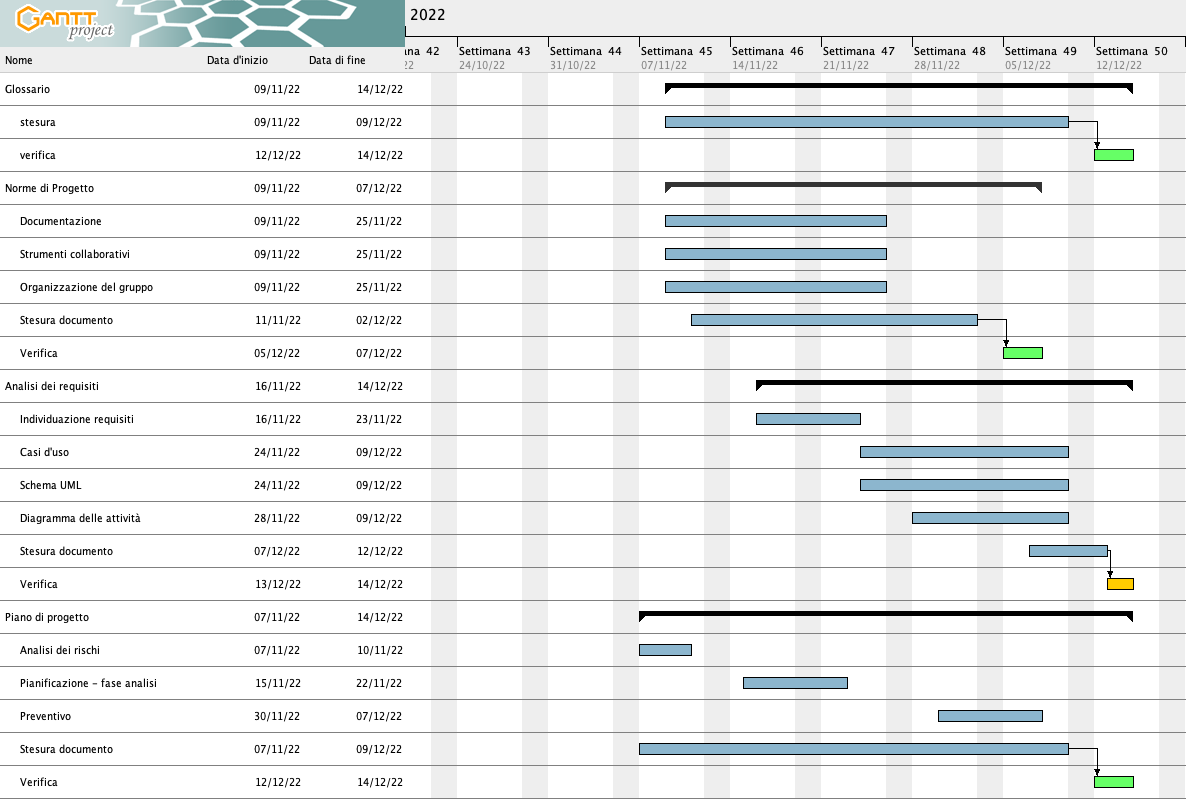
\includegraphics[scale=0.38]{image/analisi_preliminare_gantt.png}
    \caption{Diagramma di Gantt\textsubscript{g} fase di Analisi preliminare}
\end{figure}
\pagebreak
%fase PoC

\subsection{Progettazione Proof of Concept\textsubscript{g}}
Questo periodo comincia al termine del periodo di Analisi preliminare e termina con l'inizio della codifica del Proof of Concept\textsubscript{g}.\\
\begin{center}
\textbf{periodo:} dal 15-12-2022 al 16-01-2023\\
\end{center}
Questo periodo viene dedicato al completamento delle attività arretrate, per poi concentrarsi sulla 
progettazione e iniziare la codifica del Proof of Concept\textsubscript{g}. Si va inoltre avanti con la stesura 
della documentazione. Questo periodo viene suddiviso nelle attività trattate nella seguente sezione.

\subsubsection{Attività}
\begin{itemize}
\item \textbf{\textit{Glossario}:} il documento viene costantemente aggiornato con nuovi termini;
\item \textbf{\textit{Piano di Progetto}:} viene aggiunta la pianificazione del periodo, il preventivo e il consultivo;  
\item \textbf{Analisi dei requisti:} si continua la stesura del documento, completando le attività arretrate dal periodo precedente;
\item \textbf{\textit{Piano di Qualifica}:} documento nel quale vengono stabiliti gli standard di qualità di processo\textsubscript{g} e di prodotto\textsubscript{g};
\item \textbf{\textit{Norme di Progetto}:} vengono aggiunte nuove norme relative alla documentazione e alle metriche utilizzate nel \textit{Piano di Qualifica};
\item \textbf{Proof of Concept\textsubscript{g}:} ogni componente del gruppo studierà individualmente le tecnologie da utilizzare, per prendere familliarità; si inizierà poi a progettare e realizzare il Proof of Concept\textsubscript{g}, una versione semplice, ma dimostrativa, del prodotto\textsubscript{g} finale, per 
capire se è fattibile e darne una prova al proponente\textsubscript{g}.
\end{itemize}

\subsubsection{Periodi}
La Progettazione Proof of Concept\textsubscript{g} sarà suddivisa nei seguenti periodi:
\begin{itemize}
\item \textbf{Periodo 1:} \textit{dal 15-12-2022 al 21-12-2022}, pianificazione del periodo corrente con relativo preventivo, completamento attività arretrate 
(stesura del documento \textit{Analisi dei Requisiti}). Continua lo studio individuale delle tecnologie da utilizzare;
\item \textbf{Periodo 2:} \textit{dal 22-12-2022 al 04-01-2023}, inizia la stesura del documento \textit{Piano di Qualifica}. Inizia la progettazione del Proof of Concept\textsubscript{g}, si continua la stesura e la verifica\textsubscript{g} dei documenti;
\item \textbf{Periodo 3:} \textit{dal 05-01-2023 al 16-01-2023}, continua la progettazione e inizia la codifica del Proof of Concept\textsubscript{g}. Si procede nella stesura e nella verifica\textsubscript{g} della documentazione.
\end{itemize}

\begin{figure}[H]
    \centering
    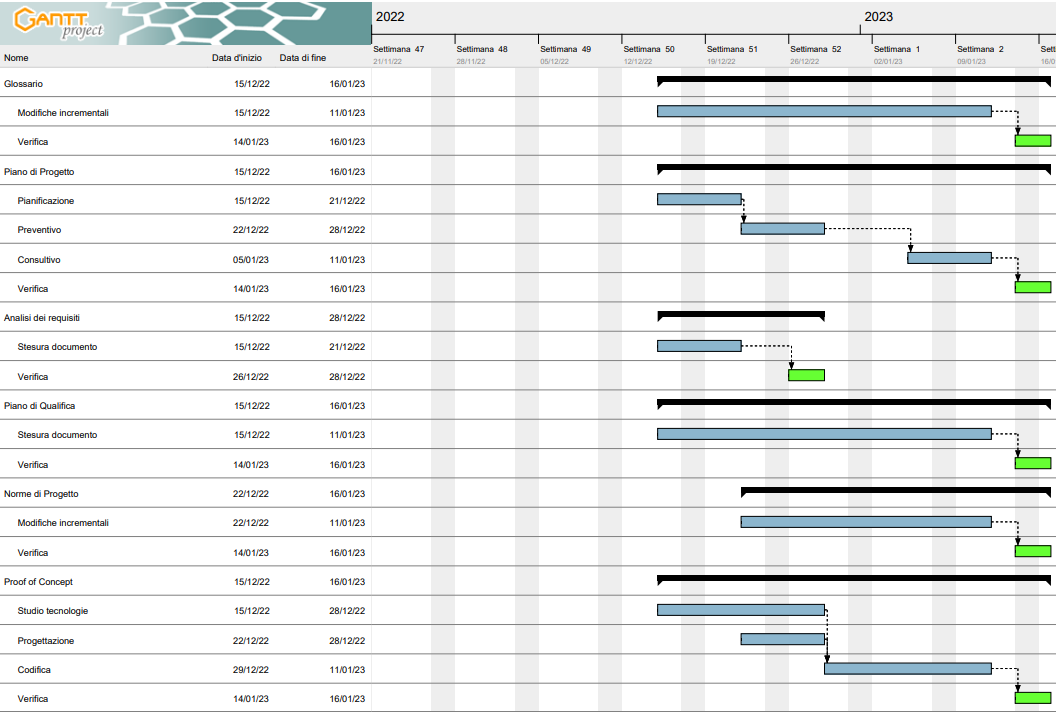
\includegraphics[scale=0.72]{image/gantt_poc.png}
    \caption{Diagramma di Gantt\textsubscript{g} fase di Progettazione Proof of Concept\textsubscript{g}}
\end{figure}
\pagebreak

\subsection{Codifica Proof of Concept\textsubscript{g}}
Questo periodo comincia al termine del periodo di Progettazione Proof of Concept\textsubscript{g} e termina con 
la consegna dei documenti per la Requirements and Tecnology Baseline.\\
\begin{center}
\textbf{periodo:} dal 17-01-2023 al 15-02-2023\\
\end{center}
In questo periodo ci si concentra sul portare a termine la codifica del Proof of Concept\textsubscript{g}, viene completata la stesura della documentazione, che 
viene alla fine approvata per la RTB. 

\subsubsection{Attività}
\begin{itemize}
\item \textbf{\textit{Glossario}:} il documento viene costantemente aggiornato con nuovi termini;
\item \textbf{\textit{Piano di Progetto}:} viene aggiunta la pianificazione del periodo, il preventivo e il consultivo;  
\item \textbf{Analisi dei Requisti:} si termina la stesura del documento applicando le modifiche necessarie;
\item \textbf{\textit{Piano di Qualifica}:} si continua con la stesura del documento;
\item \textbf{\textit{Norme di Progetto}:} viene cambiato l'indice del documento per avere una conformità con il \textit{Piano di Qualifica}, 
si completa la stesura delle sezioni mancanti;
\item \textbf{Proof of Concept\textsubscript{g}:} si completa la codifica del PoC\textsubscript{g}, aggiungendo le funzionalità stabilite in accordo con il proponente\textsubscript{g}.
\end{itemize}

\subsubsection{Periodi}
Il periodo di Codifica Proof of Concept\textsubscript{g} sarà suddivisa nei seguenti periodi:
\begin{itemize}
\item \textbf{Periodo 1:} \textit{dal 17-01-2023 al 31-01-2023}, pianificazione del periodo corrente con relativo preventivo, si continua la codifica 
del Proof of Concept\textsubscript{g}. Prosegue la stesura del \textit{Piano di Qualifica} aggiornando le metriche da seguire; si aggiornano le \textit{Norme di Progetto} di conseguenza;
\item \textbf{Periodo 2:} \textit{dal 01-02-2023 al 15-02-2023},  viene completata la codifica del PoC\textsubscript{g} e la stesura della documentazione. 
Si verifica\textsubscript{g} nel \textit{Piano di Qualifica} che le metriche siano rispettate. Si verificano e approvano tutti i documenti in previsione della RTB.
\end{itemize}

\begin{figure}[H]
    \centering
    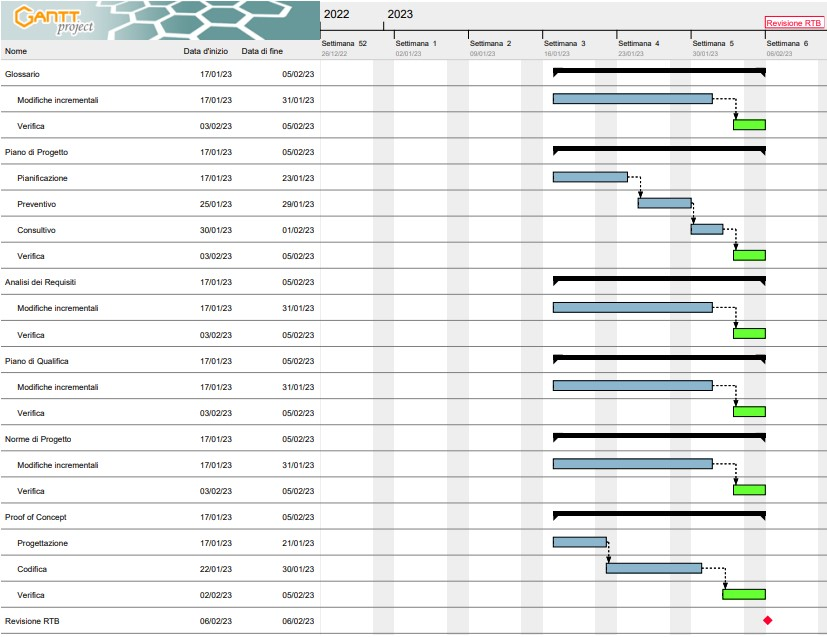
\includegraphics[scale=0.56]{image/gantt_terzo_periodo.png}
    \caption{Diagramma di Gantt\textsubscript{g} fase di Codifica Proof of Concept\textsubscript{g}}
\end{figure}
\pagebreak

\subsection{Progettazione di dettaglio e codifica dei requisiti}
Questo periodo inizia subito dopo la revisione di Requirements and Technology Baseline (RTB\textsubscript{g}) e si conclude con l'avvio della Validazione e Collaudo. Non procederemo con un aggiornamento diretto del nostro PoC\textsubscript{g}, ma piuttosto utilizzeremo il suo codice per creare una versione migliore utilizzando ulteriori librerie introdotte per facilitare l’implementazione dei pattern architetturali.
\begin{center}
\textbf{periodo:} dal 29-03-2023 al 03-05-2023\\
\end{center}
\subsubsection{Attività}
\begin{itemize}
\item \textbf{Documentazione:} stesura o modifiche ai documenti;
\item \textbf{Codifica:} produzione di codice o attività inerenti;
\item \textbf{UML\textsubscript{g}:} creazione dei diagrammi UML\textsubscript{g} o attività inerenti;  
\item \textbf{Test:} creazione dei test di unità e di integrazione;
\item \textbf{Manuali:} stesura dei manuali.
\end{itemize}
% ====================================================== SPRINT 1
\subsubsection{Sprint 1}
\begin{center}
\textbf{periodo:} dal 29-03-2023 al 05-04-2023\\
\end{center}
In questo sprint\textsubscript{g} in gruppo si concentra sulla correzione dei documenti dopo le segnalazioni dei committenti alla revisione di avanzamento RTB.
Si inizia anche ad individuare dei pattern architetturali adeguati e a studiare le librerie di interesse. Le task assegnate per questo sprint sono:
\begin{longtable}{ 
	>{\centering}M{0.30\textwidth} 
	>{\centering}M{0.10\textwidth}
	>{\centering}M{0.20\textwidth}
	}
	\rowcolorhead
	\centering 
	\headertitle{Task} &	
	\headertitle{Priorità} &
	\headertitle{Attività}
	\endfirsthead	
	\endhead
	
	Apprendimento librerie & Media & Codifica\tabularnewline
	Individuazione pattern architetturali & Media & UML\tabularnewline
	Correzione Piano di Qualifica & Bassa & Documentazione\tabularnewline
	Modello di sviluppo nel Piano di Progetto & Alta & Documentazione\tabularnewline
	Pianificazione sprint nel Piano di Progetto & Alta & Documentazione\tabularnewline
	Preventivo dello sprint nel Piano di Progetto & Alta & Documentazione\tabularnewline
	Diario di Bordo & Bassa & Documentazione\tabularnewline
	Verbale & Bassa & Documentazione\tabularnewline
	Correzione Norme di Progetto & Media & Documentazione\tabularnewline
	\captionline \caption{Task assegnate nello sprint 1}
\end{longtable}


\begin{figure}[H]
    \centering
    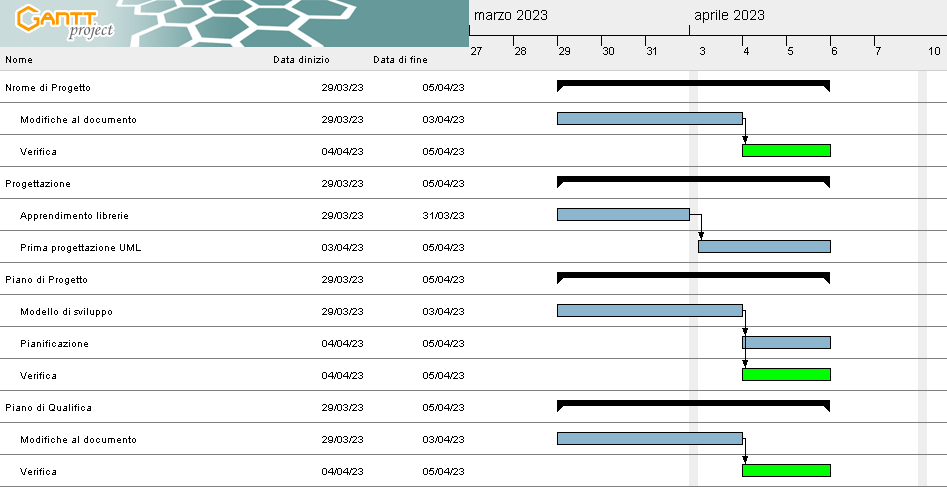
\includegraphics[scale=0.56]{image/gantt_sprint1.PNG}
    \caption{Diagramma di Gantt\textsubscript{g} Sprint\textsubscript{g} 1}
\end{figure}
% ====================================================== SPRINT 2
\subsubsection{Sprint 2}
\begin{center}
\textbf{periodo:} dal 06-04-2023 al 13-04-2023\\
\end{center}
In questo sprint\textsubscript{g} il gruppo si concentra a produrre un possibile diagramma delle classi. 
Nel caso avanzino ore lavorative ci occuperemo della produzione di un possibile diagramma di sequenza e di iniziare la stesura delle norme
di codifica.

Le task assegnate per questo sprint sono:
\begin{longtable}{ 
	>{\centering}M{0.30\textwidth} 
	>{\centering}M{0.10\textwidth}
	>{\centering}M{0.20\textwidth}
	}
	\rowcolorhead
	\centering 
	\headertitle{Task} &	
	\headertitle{Priorità} &
	\headertitle{Attività}
	\endfirsthead	
	\endhead
	
	Diagramma delle classi & Alta & UML\tabularnewline
	Diario di Bordo del 10-04-2023 & Alta & Documentazione\tabularnewline
	Verbale del VI\_06-04-2023 & Alta & Documentazione\tabularnewline
	Verbale del VE\_05-04-2023 & Alta & Documentazione\tabularnewline
	Pianificazione sprint 3 & Alta & Documentazione\tabularnewline
	Diagramma di sequenza & Media & UML\tabularnewline
	Norme sulla codifica & Media & Documentazione\tabularnewline
	
\end{longtable}

\begin{figure}[H]
	\centering 
	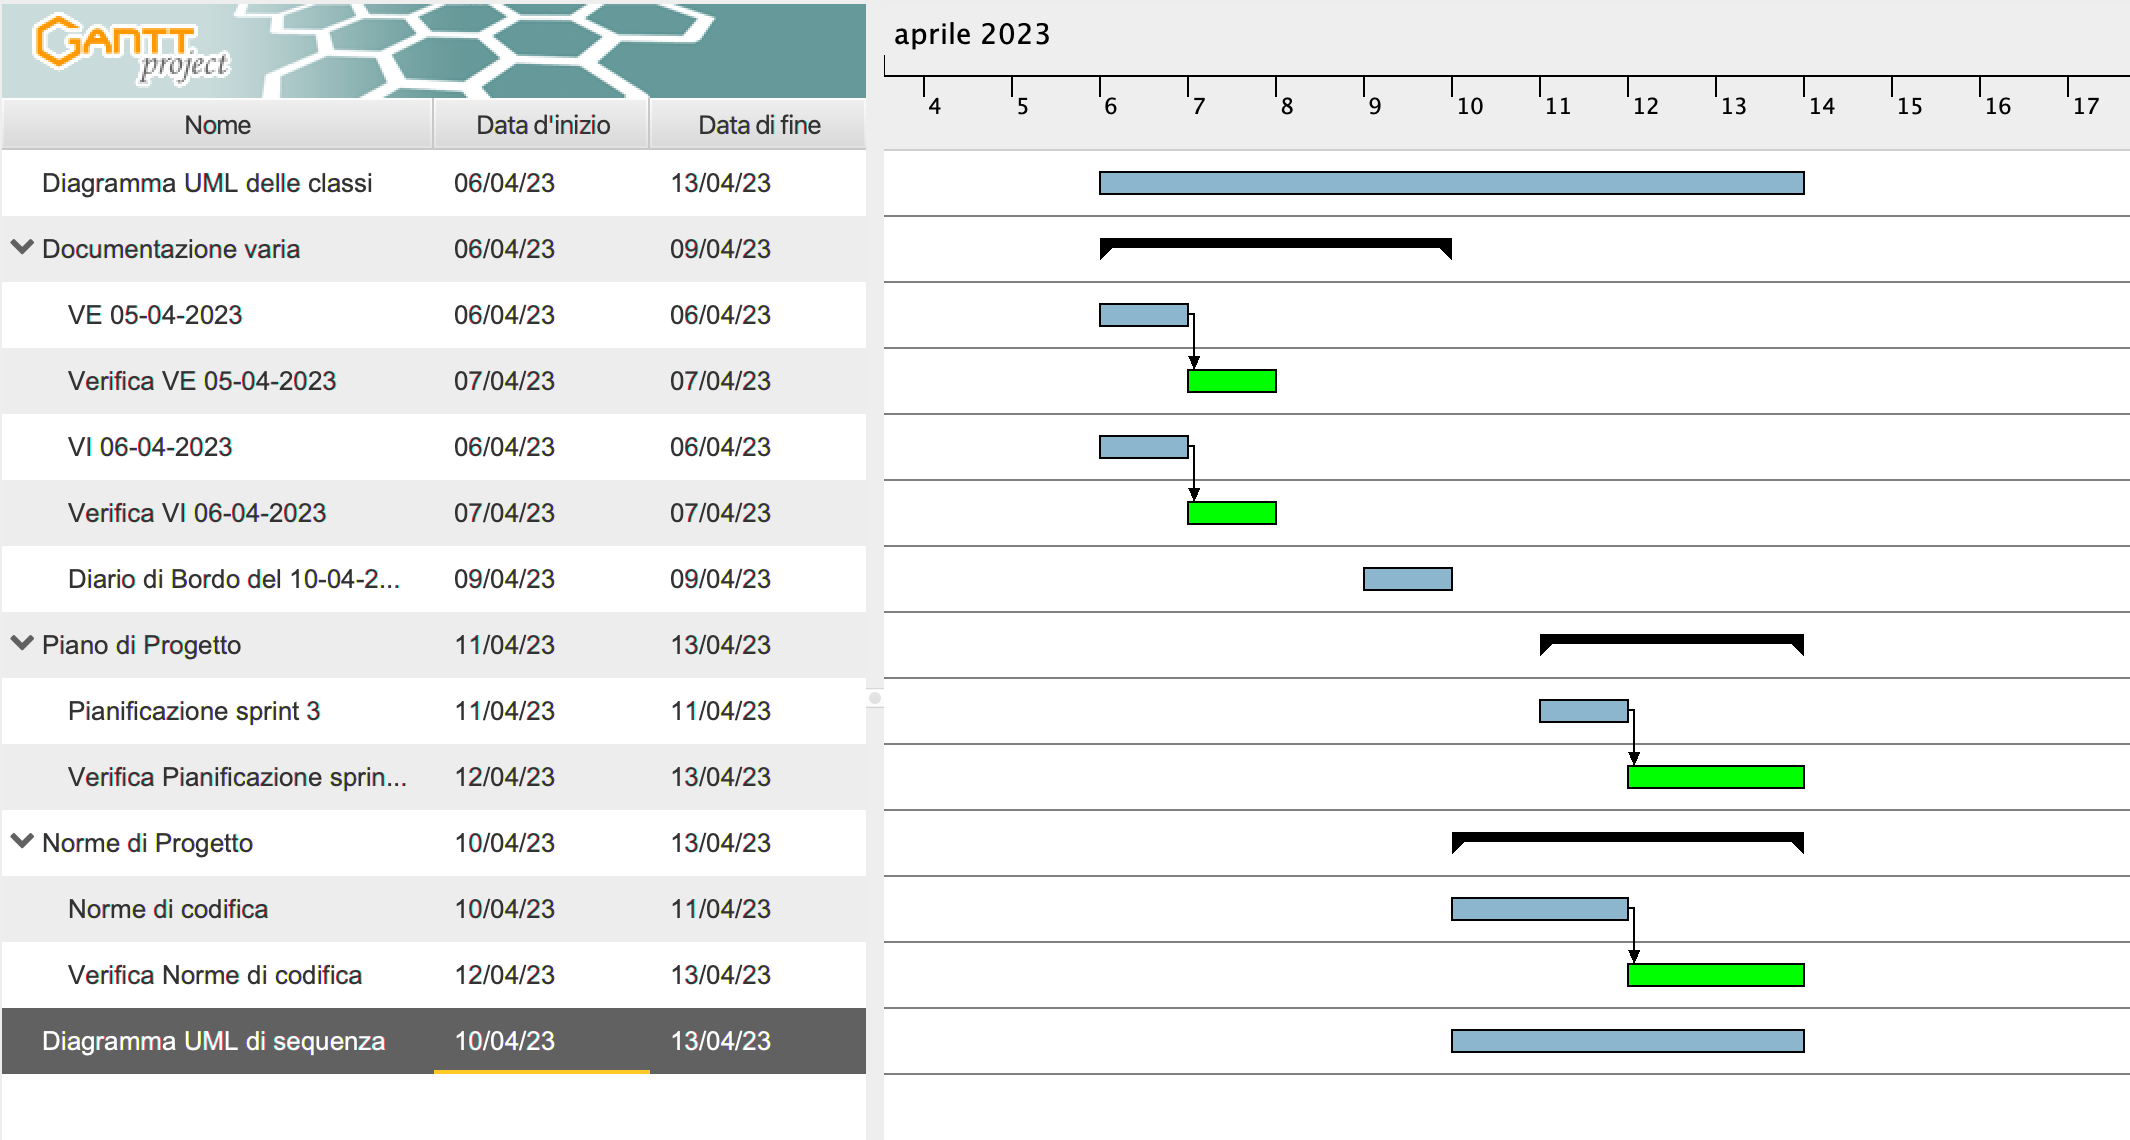
\includegraphics[scale=0.42]{image/gantt_sprint2.PNG}
	\caption{Diagramma di Gantt\textsubscript{g} Sprint\textsubscript{g} 2}
\end{figure}
\pagebreak
% ====================================================== SPRINT 3
\subsubsection{Sprint 3}
\begin{center}
\textbf{periodo:} dal 14-04-2023 al 21-04-2023\\
\end{center}
In questo sprint\textsubscript{g} verranno richiesti dei chiarimenti al Professor Riccardo Cardin sul diagramma delle classi prodotto.
Successivamente il gruppo si concentra a provare l'esattezza del diagramma delle classi prodotto tramite una prima codifica esplorativa per tornare a correggere
il diagramma nel caso verranno trovati degli errori di progettazione o aspetti che vanno migliorati.


Le task assegnate per questo sprint sono:
\begin{longtable}{ 
	>{\centering}M{0.30\textwidth} 
	>{\centering}M{0.10\textwidth}
	>{\centering}M{0.20\textwidth}
	}
	\rowcolorhead
	\centering 
	\headertitle{Task} &	
	\headertitle{Priorità} &
	\headertitle{Attività}
	\endfirsthead	
	\endhead
	
	Norme di codifica & Alta & Documentazione\tabularnewline
	Norme sui test di unità & Alta & Documentazione\tabularnewline
	Norme sui test di integrazione & Alta & Documentazione\tabularnewline
	Scena base & Media & Codifica\tabularnewline
	Movimenti player & Media & Codifica\tabularnewline
	Aggiornamento analisi dei rischi Piano di Progetto & Bassa & Documentazione\tabularnewline
	Aggiunta sezione introduzione Piano di Progetto & Bassa & Documentazione\tabularnewline
	VE\_14-04-2023 & Bassa & Documentazione\tabularnewline
	Pianificazione Sprint 4 & Bassa & Documentazione\tabularnewline
	
\end{longtable}

\begin{figure}[H]
	\centering 
	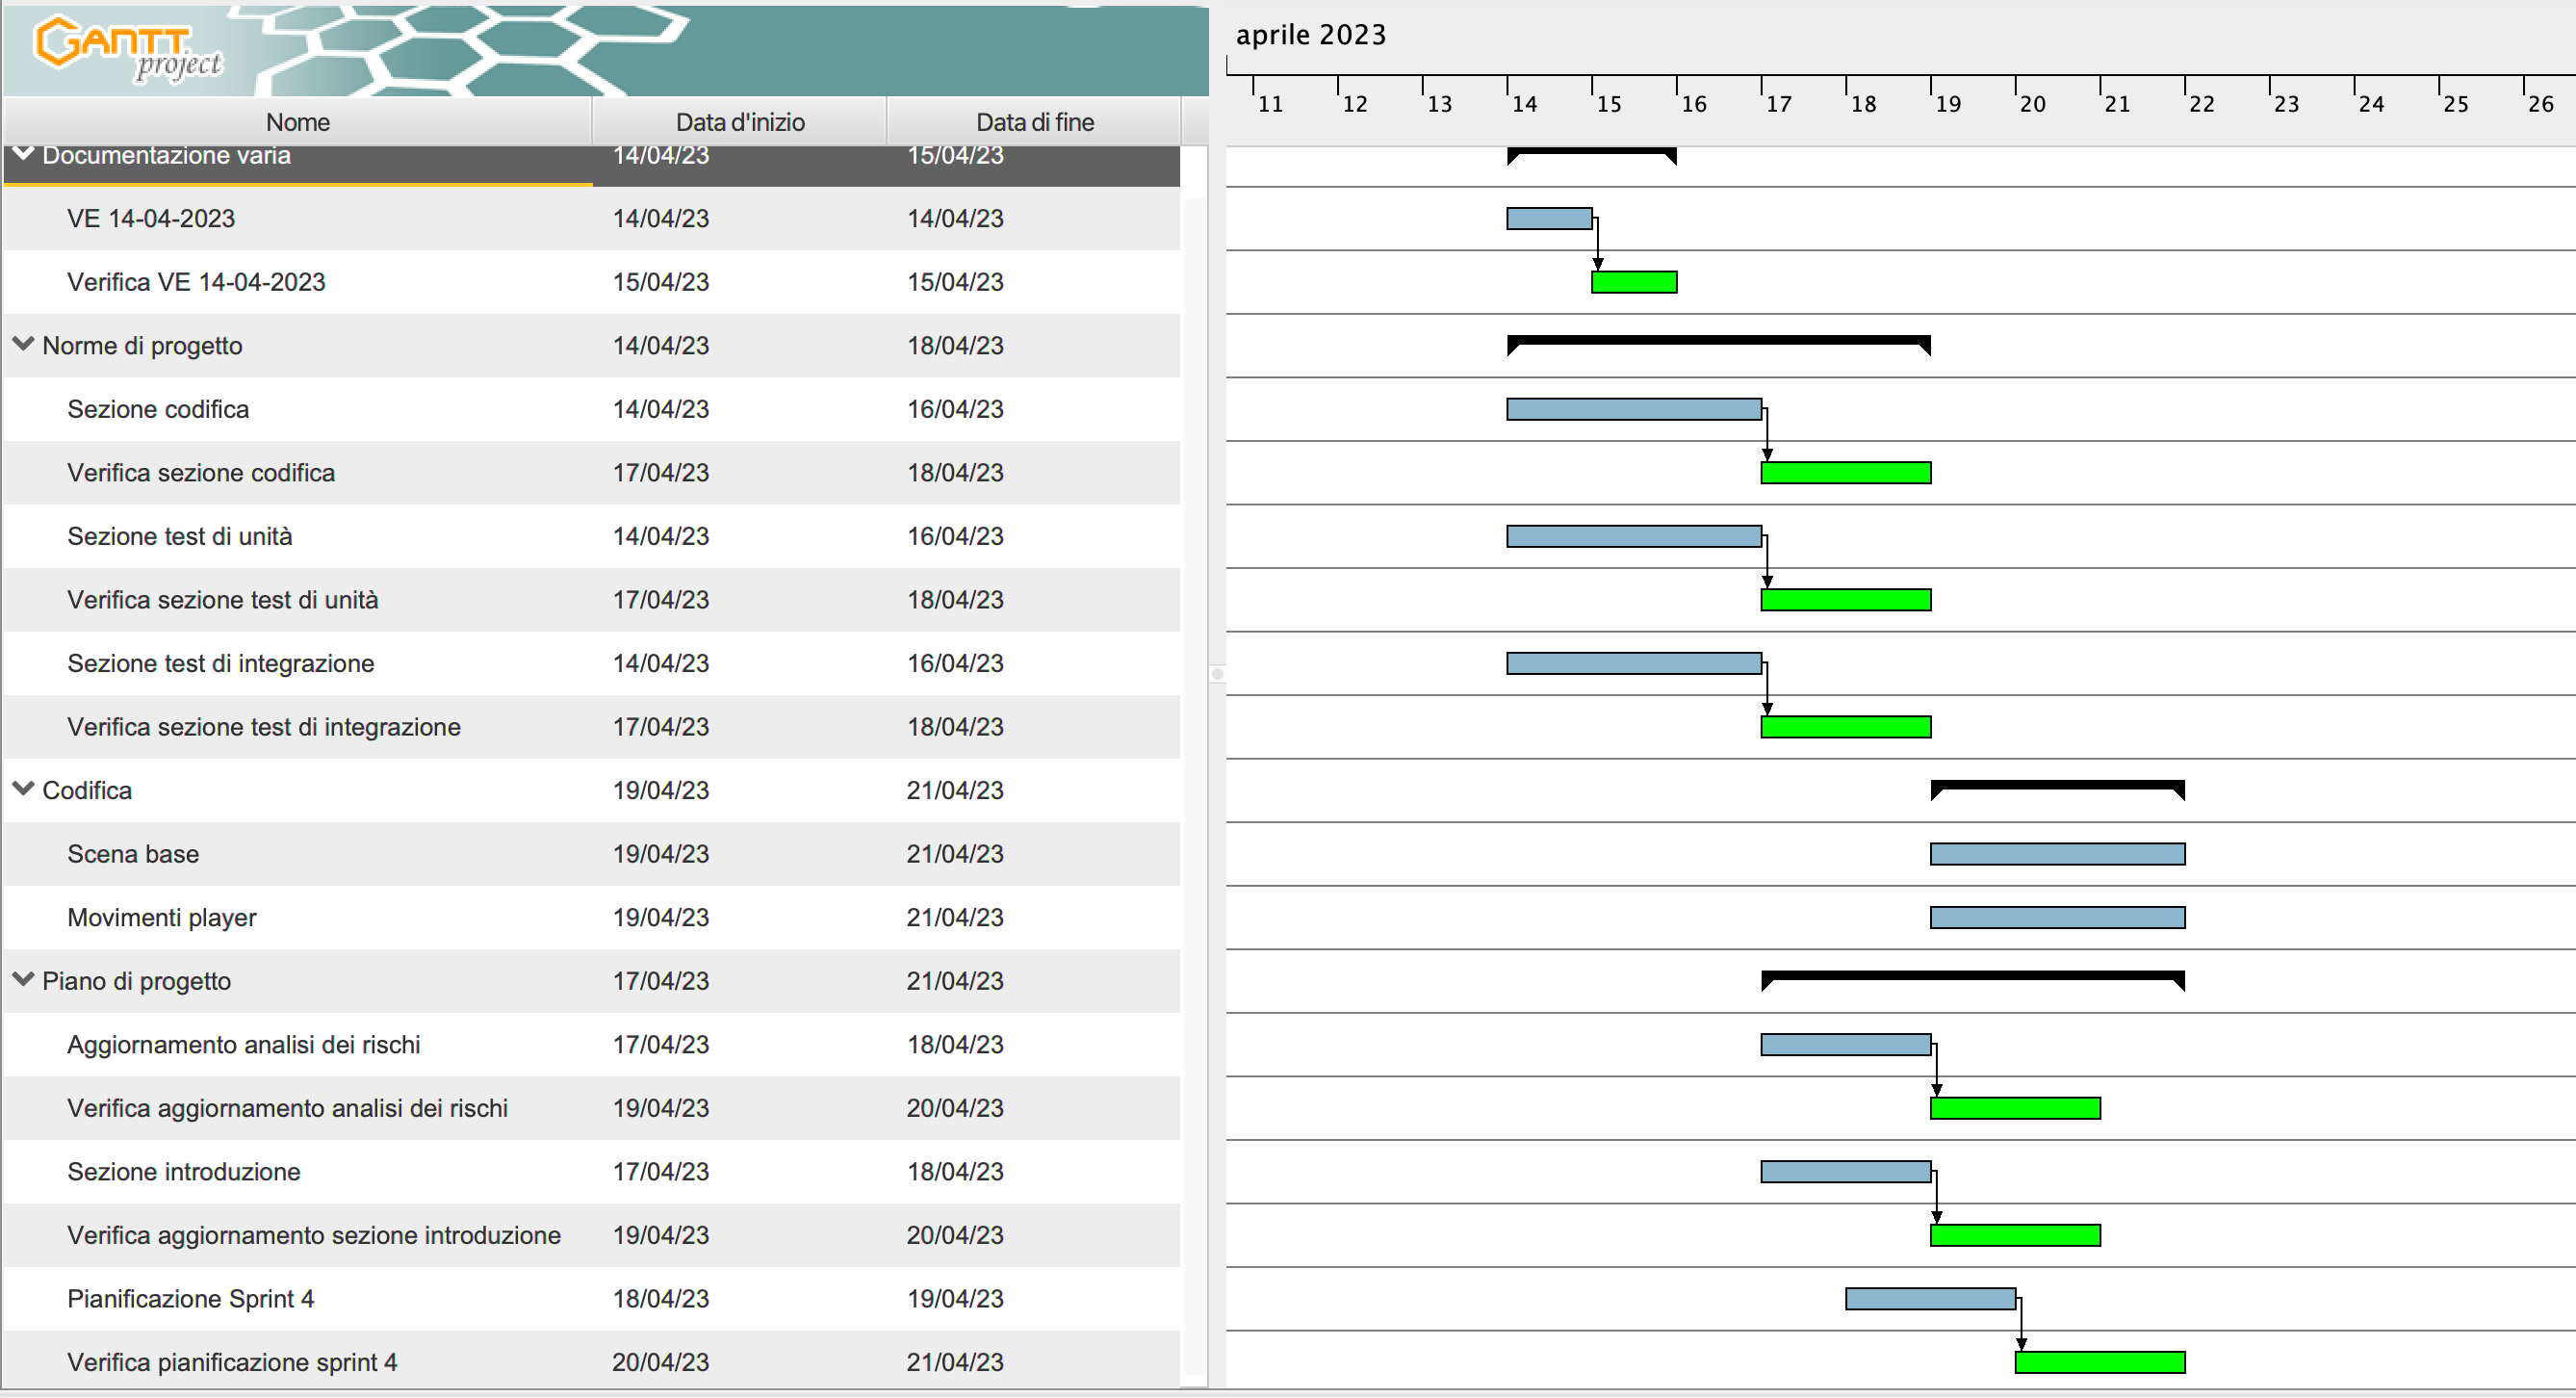
\includegraphics[scale=0.32]{image/gantt_sprint3.PNG}
	\caption{Diagramma di Gantt\textsubscript{g} Sprint\textsubscript{g} 3}
\end{figure}
\pagebreak
% ====================================================== SPRINT 4
\subsubsection{Sprint 4}
\begin{center}
\textbf{periodo:} dal 22-04-2023 al 03-05-2023\\
\end{center}
In questo sprint\textsubscript{g} ci concentreremo soprattutto sulla codifica e il consolidamento delle norme di codifica, di test e diagramma delle classi.
Dopo aver sviluppato una parte dell'applicazione verrà contattato il proponente per chiedere un parere sull' esperienza utente e per far vedere quanto prodotto dalla codifica.
Contatteremo anche il Professor Riccardo Cardin per far vedere le modifiche che secondo noi possono essere definitive apportate al diagramma delle classi.
Alla fine di questo sprint\textsubscript{g} ci aspettiamo di aver raggiunto un buon punto nello sviluppo dell'applicazione.
Probabilmente sarà necessario uno sprint ulteriore per concludere il progetto in quanto lo sprint 4 non prevede la stesura dei manuali e 
della documentazione necessaria a candidarsi alla revisione TB.
Nel caso si verificassero imprevisti personali o modifiche all'applicazione verrà tenuto in considerazione di aggiungere più di uno sprint.
A questo punto ci rendiamo conto che non sarà possibile soddisfare i requisiti opzionali in quanto il gruppo non dispone del monte ore e budget
necessario.

Le task assegnate per questo sprint sono:
\begin{longtable}{ 
	>{\centering}M{0.30\textwidth} 
	>{\centering}M{0.10\textwidth}
	>{\centering}M{0.20\textwidth}
	}
	\rowcolorhead
	\centering 
	\headertitle{Task} &	
	\headertitle{Priorità} &
	\headertitle{Attività}
	\endfirsthead	
	\endhead
	
	Norme sull'integrazione continua & Alta & Documentazione\tabularnewline
	Pianificazione Sprint 5  & Media & Documentazione\tabularnewline
	Diario di Bordo del 24-04-2023 & Media & Documentazione\tabularnewline
	Diario di Bordo del 01-05-2023 & Media & Documentazione\tabularnewline
	Norme di codifica & Alta & Documentazione\tabularnewline
	Norme di test & Alta & Documentazione\tabularnewline
	Codifica scena base & Alta & Codifica\tabularnewline
	Codifica movimenti player & Alta & Codifica\tabularnewline
	
	
\end{longtable}

\begin{figure}[H]
	\centering 
	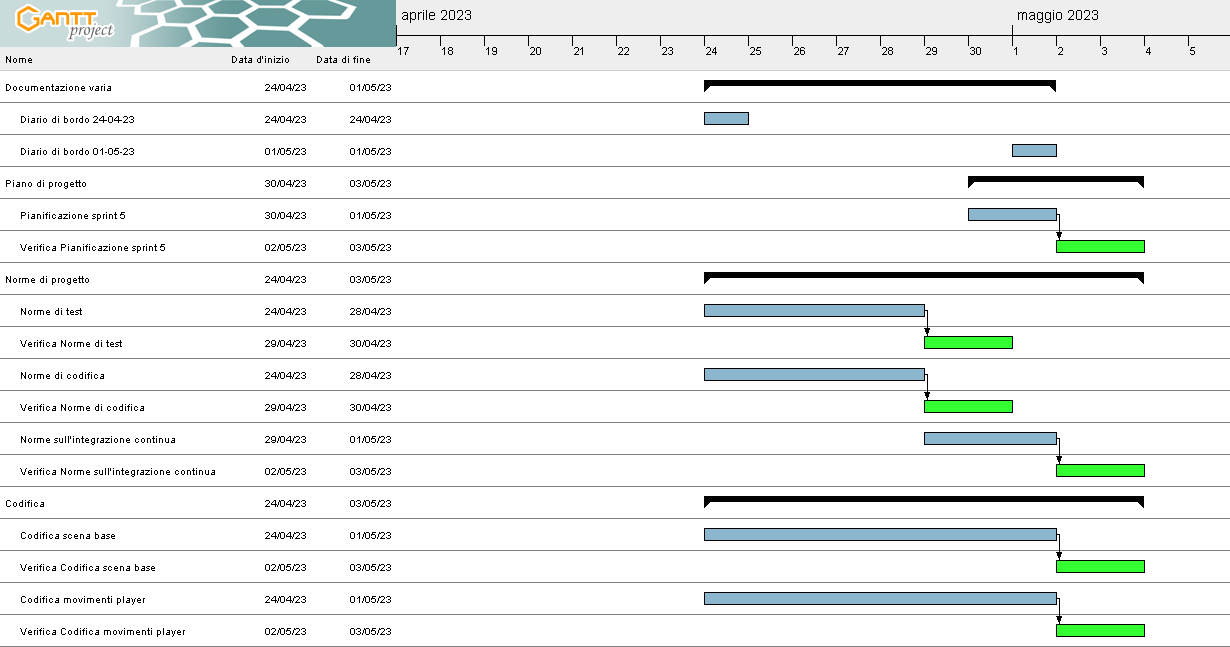
\includegraphics[scale=0.37]{image/gantt_sprint4.PNG}
	\caption{Diagramma di Gantt\textsubscript{g} Sprint\textsubscript{g} 4}
\end{figure}
\pagebreak% ====================================================== SPRINT 5
\subsubsection{Sprint 5}
\begin{center}
\textbf{periodo:} dal 03-05-2023 al 17-05-2023\\
\end{center}
In questo sprint\textsubscript{g} ci concentreremo soprattutto sulla codifica delle componenti principali e il consolidamento delle norme riguardanti i documenti di specifica tecnica e manuale utente.
Alla fine di questo sprint\textsubscript{g} ci aspettiamo di aver sviluppato, se non tutte, la maggior parte delle funzionalità del prodotto.

Le task assegnate per questo sprint sono:
\begin{longtable}{ 
	>{\centering}M{0.30\textwidth} 
	>{\centering}M{0.10\textwidth}
	>{\centering}M{0.20\textwidth}
	}
	\rowcolorhead
	\centering 
	\headertitle{Task} &	
	\headertitle{Priorità} &
	\headertitle{Attività}
	\endfirsthead	
	\endhead
	
	Norme sul manuale utente & Alta & Documentazione\tabularnewline
	Norme sulla specifica tecnica  & Alta & Documentazione\tabularnewline
	Pianificazione Sprint 6  & Media & Documentazione\tabularnewline
	Codifica delle slice & Alta & Codifica\tabularnewline
	Codifica dei componenti UI & Alta & Codifica\tabularnewline
	Codifica test di unità & Alta & Codifica\tabularnewline
	Diario di Bordo del 08-05-2023 & Media & Documentazione\tabularnewline
	Diario di Bordo del 15-05-2023 & Media & Documentazione\tabularnewline
	
	
\end{longtable}

\begin{figure}[H]
	\centering 
	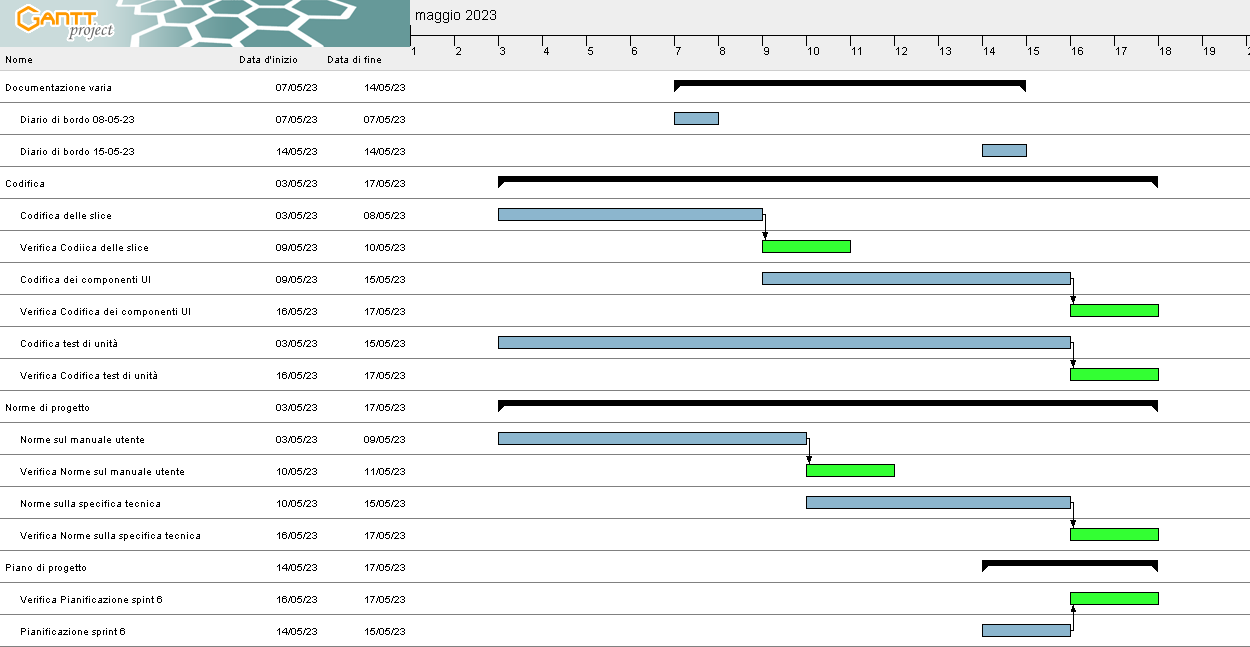
\includegraphics[scale=0.37]{image/gantt_sprint5.PNG}
	\caption{Diagramma di Gantt\textsubscript{g} Sprint\textsubscript{g} 5}
\end{figure}
\pagebreak% ====================================================== SPRINT 6
\subsubsection{Sprint 6}
\begin{center}
\textbf{periodo:} dal 17-05-2023 al 07-06-2023\\
\end{center}
In questo sprint\textsubscript{g} verranno concluse le attività di codifica e stesura di documentazione. \\
Si pianifica di raggiungere la baseline successiva al termine di questo sprint.

Le task assegnate per questo sprint sono:
\begin{longtable}{ 
	>{\centering}M{0.30\textwidth} 
	>{\centering}M{0.10\textwidth}
	>{\centering}M{0.20\textwidth}
	}
	\rowcolorhead
	\centering 
	\headertitle{Task} &	
	\headertitle{Priorità} &
	\headertitle{Attività}
	\endfirsthead	
	\endhead
	
	Consuntivo finale & Media & Documentazione\tabularnewline
	Norme manuale utente  & Alta & Documentazione\tabularnewline
	Specifica tecnica & Alta & Documentazione\tabularnewline
	Manuale utente  & Alta & Documentazione\tabularnewline
	Norme specifica tecnica & Alta & Documentazione\tabularnewline
	Aggiunta nuovi modelli 3D & Alta & Codifica\tabularnewline
	Codifica torcia & Alta & Codifica\tabularnewline
	Codifica sidebar & Alta & Codifica\tabularnewline
	Diario di Bordo del 22-05-2023 & Media & Documentazione\tabularnewline
	Diario di Bordo del 29-05-2023 & Media & Documentazione\tabularnewline
	Diario di Bordo del 05-06-2023 & Media & Documentazione\tabularnewline
	
	
\end{longtable}

\begin{figure}[H]
	\centering 
	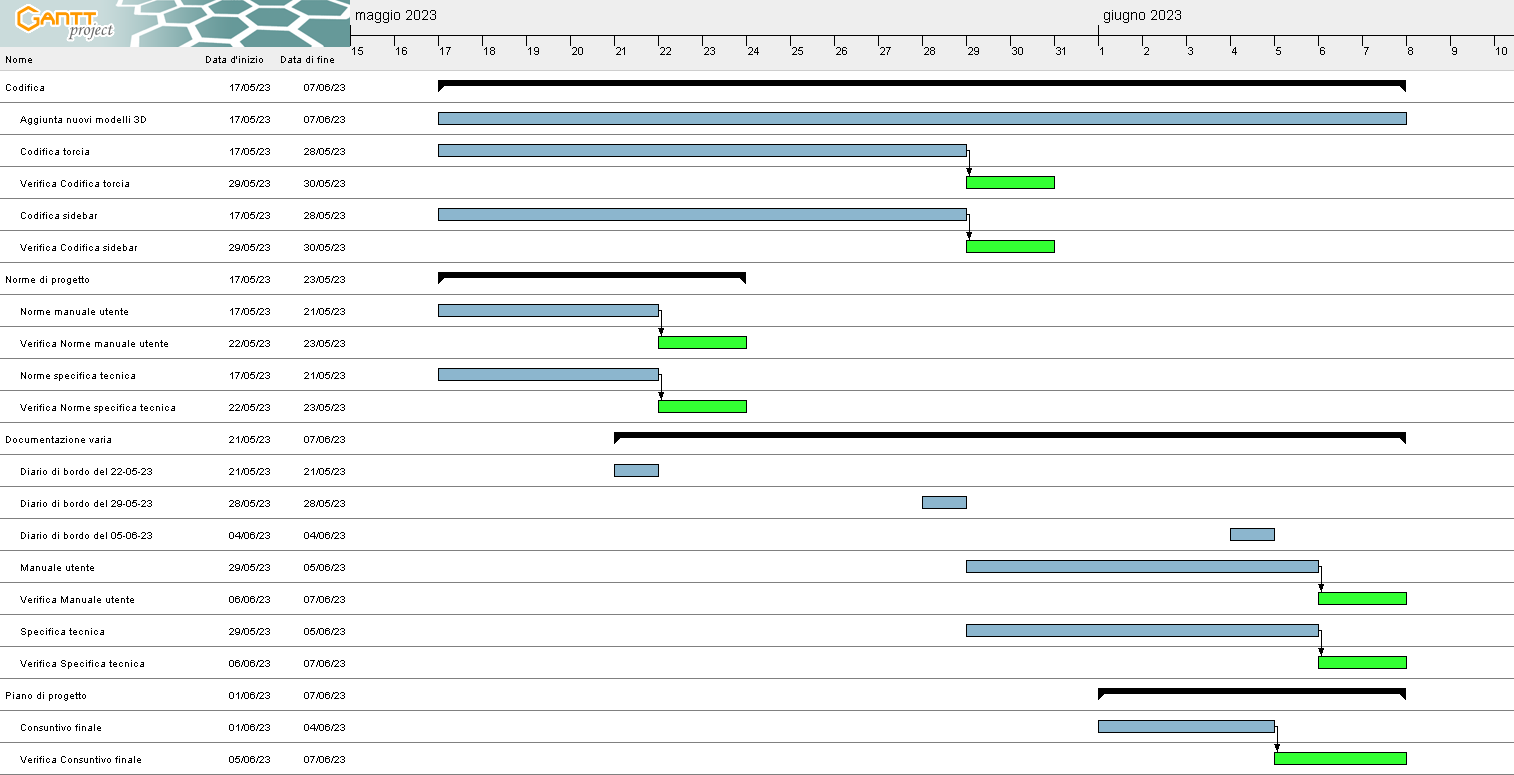
\includegraphics[scale=0.32]{image/gantt_sprint6.PNG}
	\caption{Diagramma di Gantt\textsubscript{g} Sprint\textsubscript{g} 6}
\end{figure}
\pagebreak